
\chapter{“Hinduism: a Precursor to Nazism?”}\index{Nazism}\label{chapter8}

\Authorline{-- Vishal Agarwal$^{\ast}$}\footnotetext{*pp.~\pageref{chapter8}\enginline{--}\pageref{chapter8-end}. In: Kannan, K. S and Meera, H. R. (Ed.s) (2021). \textit{Chronology and Causation: Negating Neo-Orientalism.} Chennai: Infinity Foundation India.}

\lhead[{\small\thepage}\quad\small Vishal Agarwal]{}

\begin{flushright}
\textit{(vishalsagarwal@yahoo.com)}
\end{flushright}

\setcounter{endnote}{0}

\section*{1. Orientalism, National Socialism\index{National Socialism} and the Aryan Race:}\index{Aryan race}

By the late nineteenth century, Orientalist scholarship on India began to act as the handmaiden of European colonialism and imperialism by pretending that it had discovered and understood the roots of colonized cultures like Indian culture. It sought to demarcate the strata of texts of the Indian civilization to search for ‘external influences and later accretions’ and map them to the ‘different races that populated India.’ The ‘natives’ of India were classified as various degrees of mongrel peoples due to the admixture of the superior, virile, civilized invading ‘Aryans’ from the northwest (closer to Europe) and the effeminate, inferior, dark skinned and less civilized indigenous Indians. But this is not how Oriental scholarship started, or evolved in other parts of the world.

In the early eighteenth century in Germany, Friedrich von Schlegel\index{Schlegel, Friedrich von} had proposed that a master Aryan race had originated from the Himalayas and migrated to various parts of Europe with their knowledge in antiquity. Their language, closely related to Sanskrit, was called ‘Indo-Germanic family of languages’ and later as ‘Indo-European’. Georg Hegel\index{Hegel, Georg} and Christian Lassen\index{Lassen, Christian} propagated this myth, but Schlegel’s brother Wilhelm later relocated the Aryan homeland to Caucasus, from where they had invaded India (Kennedy 2000:81-82). Developments in historical linguistics led to a mapping of languages to ‘races’, with the Indo-European languages being linked to the ‘Aryans’ by other European scholars like Max Mueller\index{Müller, Max} and Joseph Renan.\index{Renan, Joseph} This ‘Aryan Myth’ distinguished sharply between the ‘Aryan Race’\index{Aryan race} and the ‘Semitic Race’ (Jews), thereby ‘othering’\index{othering} the already ‘outsider’ Jews in Europeans. Many European scholars however found the natural conclusion that Christianity\index{Christianity} was ‘Semitic’ despite their own ‘Aryan’ racial affiliation as unpalatable. In particular, the British could not digest the fact that they shared racial affinity with Indians colonized by them, except with perhaps the elite Brāhmaṇas\index{brahmana@\textit{brāhmaṇa}} among the Hindus. The French aristocrat Joseph Gobineau,\index{Gobineau, Joseph} and the Englishman Houston Chamberlain\index{Chamberlain, Houston} further transformed the Aryan Myth into a thesis of Nordic-Teutonic racial supremacy in the period after 1850 CE. These Nordics were considered as ‘pure Aryans’, blonde and blue eyed. The rise of German Nationalism after the Franco-Prussian war contributed to the popularity of the Nordic Aryan thesis amongst Germans, who believed themselves as the purest descendants and true representatives of this master race (Kennedy\index{Kennedy, Kenneth} 2000:82-83).

In the early 20th century, fringe lunatics like G. Lanz-Liebehfels took this Nordic Aryan thesis further and launched a journal \textit{Istara}, of which Hitler is said to have been a regular reader (Halbfass\index{Halbfass, Wilhelm} 1988:139-140). It was Lanz who termed the Swastika as an Aryan symbol,\endnote{ The official emblem of Nazis, the ‘Swastika’ was adopted by Hitler himself, who declared in his Mein Kampf, that represented, “…the fight for the victory of the Aryan man and at the same time for the victory of the idea of creative work, which in itself always was and always will be anti-Semitic.” (Cited in Murphy \textit{et al}, p. 87). There is really nothing particularly Aryan about Swastika, as it is attested even in Harappan contexts (deemed as ‘pre-Vedic’ by Indologists) as well as in African and many other cultures.} and also highlighted the contrast between the dark \textit{caṇḍāla} and the blonde Aryan. Developing these ideas further, Alfred Rosenberg wrote his ‘\textit{Der Mythus der 20 Jahrunderts}’ which became the official ideology of National Socialism\index{National Socialism}, more popularly known as Nazism\index{Nazism}. It envisaged the Germans as the least mongrel, and therefore the pre-esteemed and creative members of the superior Nordic Aryan race. Alfred Rosenberg, the high priest of the Nazi racial theory wrote,

\begin{myquote}
“The meaning of world history has radiated out from the north over the whole world, borne by a blue-eyed blond race which in several great ways determined the spiritual face of the world….These wander-periods were the legendary migration of the Atlatindes across north Africa, the migration\index{Aryan Migration Theory} of the Aryans into India and Persia; the migrations of the Dorians, Macedonians, Latins; the migration of the Germanic tribes; the colonization of the world of the Germanic occident.”\endnote{ Rosenberg\index{Rosenberg, Alfred} himself preferred the word “Nordic” to “Aryan”, unlike other Nazi ideologues. In fact, “Aryan” and its cognates are scarcely attested in non-Indo-Iranian languages.} 

~\hfill Cited in Murphy \textit{et al }(1952: 71)
\end{myquote}

Rosenberg\index{Rosenberg, Alfred} then elaborated on each individual migration as to how the genetic mixture of the superior Aryans with the non-Aryan ‘inferior races’ in their colonies had resulted in a degradation of civilization, because the ‘creative impulse of the Aryans’ got diluted genetically. Below the Aryans were the Mongoloids, who were termed as ‘culture bearing’, below them the ‘Blacks and Slavs’ who were of ‘lesser value’, and finally at the bottom were the Jews, who were the sheer embodiment of evil (Burleigh and Wippermann 1997: 83). Archaeologists like Kossina\index{Kossina} manipulated and even fabricated archaeological ‘evidence’ to ‘prove’ the arrival of the master Aryan race\index{Aryan race} into northern Germany from Scandinavia (see Diaz-Andreu 1996).

Nazism had a checkered relationship with Christianity.\index{Christianity}\endnote{ Within the Indian context however, Christianity\index{Christianity} aligned itself with Orientalist scholarship to project British colonialism as a ‘civilizing mission’ of the barbarian Hindu who practiced ‘evil idolatry’ and ‘oppressed the lower castes’.} Christianity was a Semitic faith from the hated non-Aryan Jews, and was meant to be replaced by a true Aryan religion (Murphy \textit{et al}.~1952: 71).\endnote{ However, Rosenberg reserved his worst animus for Catholicism,\index{Catholicism} and appreciated Lutheran Protestantism for condemning the former (Fitzgerald 2013: 22 sqq.) but nevertheless objected to Christianity not recognizing racial superiority of the Aryan race.\index{Aryan race}} Paradoxically, anti-Semitism\index{anti-Semitism} in German had another very important religious source – the writings of the founder of Protestant\index{Protestant Christianity} Christianity, Martin Luther\index{Luther, Martin} (a German), who in his \textit{The Jews and their Lies} wrote that the Jews were the killers of Christ, they desired world domination, they were ‘pestilence’, ‘criminals’, whose institutions and books ought to be burned, and who must be driven out like ‘mad dogs’ (Spielvogel 1996: 268) While Luther’s views were extreme, anti-Semitism was firmly ingrained in the medieval Christian European mind that considered the Jews as ‘Christ killers.’\endnote{ Venkat (2007) points out that the \textit{New Testament} itself has over 450 anti-Semitic references.} Hitler considered fighting against the Jews as ‘the will of the Lord’ (Spielvogel 1996: 266). If Protestantism has been implicated as a source of Nazism,\index{Nazism} Catholicism\index{Catholicism} has been excoriated as a colluder. There are allegations of Pope Pius\index{Pope Pius XII} XII negotiating with the Nazis to protect his Church, support the Nazi rise to power, and ignore the mass extermination of Jews, Gypsies and other non-Catholic Europeans.\endnote{ See Cornwell (2000). Apologists like Bergman (2012) however absolve Christianity\index{Christianity} by arguing that the Nazi Aryan Myth derived from Darwinism, that the Nazis bore an antipathy to Catholicism\index{Catholicism} in general, and that even the anti-Semitism\index{anti-Semitism} of Martin Luther\index{Luther, Martin} resulted from this illness in his last years (\textit{ibid}, pp. 306-312).}

\vspace{-.3cm}

\section*{2. German Indology, Nazism \hfill\break and Pollock’s Civilizing Mission}\index{Pollock, Sheldon}

There were not just scholars of humanities that provided the ideological props for (or looked the other way \textit{vis-à-vis}) Nazism, but also scientists (see Cornwell 2003) like the famous physicist Phillip Lenard (FitzGerald 2013), physicians (see Kater 1989) and scholars of numerous other disciplines. Some medical professionals in particular took Nazism race theories to implement eugenics,\index{eugenics} and the elimination of ‘genetically defective’ (and therefore ‘inferior’) humans like the disabled (Hamburger 1952:~108-110). Some Indologists such as Johannes Hertel\index{Hertel, Johannes} (see Frank Neubert 2004) were supporters of the Nazi National Socialist party; other Indologists such as Walther Wust\endnote{ A simple google search will reveal Wust’s deep Nazi connections but Pollock (1993) is sufficient. There are not many publications on this important subject, and when Pollock\index{Pollock, Sheldon} was writing the above article, only some German Indologists were willing to help him. See \url{https://groups.yahoo.com/neo/groups/INDOLOGY/conversations/topics/919} for this revelation.} (author of a celebrated book on Ṛgvedic chronology\index{Chronology} besides numerous other works on Indo-Iranian linguistics) actually actively engaged in enriching Nazi 'Aryan mysticism'. Then, we have Erich Frauwallner\index{Frauwallner, Erich} who showed commitment to Nazism even after the World War II was over (see Adluri\index{Adluri, Vishwa} 2011). But whereas, the German scientists and physicians have apologized for their predecessors’ collusion with Nazism,\index{Nazism} the Indologists have not yet. Scholars of Indology or Hinduism Studies continue to cite Nazi Indologists as authorities with approval.\endnote{ Conversely, their attitude towards anyone challenging their own views is to lump ‘the Hindu other’ as a ‘Hindu Nationalist’ (and by implication, a ‘Muslim killer’, and ‘Hindu Nazi’).} In any respectable field, works of these scholars would be anathema. But not so in Indology, where they are still cited with approval. For instance, Witzel\index{Witzel, Michael} quotes Wust as a former scholar approvingly in one his own publications.\endnote{ For instance, see Witzel\index{Witzel, Michael} (1995: 312).} Other European scholars have published Kliene Schriften volumes of these Nazi Indologists.\endnote{ Other Nazi Indologists include Paul Thieme. Wilhelm Hauer, Ludwig Alsdorf, Ernst Schneider, Hermann Lommel, Richard Schmidt and many others – all big names in German Indology, cited with reverence even today. See Pollock (1993).}

This troubles Sheldon Pollock\index{Pollock, Sheldon}. In his 1993 article “Deep Orientalism” written in his typical constipated prose with claims squirted in all directions like the ink of a frightened squid, Pollock laments at modern German Indology still not coming to terms with its Nazi past. But alarmingly, he takes a step forward – and argues that Orientalism on the one hand, and racism and the ‘discourse of power’ on the other, did not originate from Orientalism or its German variant (National Socialism)\index{National Socialism}. Rather, a ‘pre-modern racism’ and the ‘discourse of power’ have deep roots within the Hindu shāstric tradition. He argues that Hindu elites (the ‘Brāhmaṇas’)\index{brahmana@\textit{brāhmaṇa}} had created a discourse wherein they were superior by birth, controlled access to empowering knowledge, and had castigated the \textit{śūdra}-s\index{sudra@\textit{śūdra}} as the excluded other – just like the disenfranchised Jew in Nazi Germany. Pollock of course does not state explicitly that Hinduism is a form of Nazism, but any reader can connect the dots and conclude that this is what he is trying to say.

If Orientalism was a racist discourse of power to define the colonized and show him to be inferior and in need of the Imperialist civilizing mission, Pollock wonders if the ‘pre-modern racism’ in Hindu scriptures is a form of ‘Deep Orientalism’ too. In his thesis of ‘Deep Orientalism’ in Hinduism, Pollock projects the ‘Ārya-Mleccha’ and ‘Ārya-Śūdra’ dichotomies in Hindu scriptures as an ancient variant of the Nazi ‘Aryan-Semite’ binary. He also singles out the Dharma-śāstra and Mīmāṁsā\index{Mimamsa@Mīmāṁsā}/Vedānta traditions for their alleged ‘discourse of power’ and exclusion of the Indian masses comprising of \textit{śūdra}-s, women, Buddhists and Jains.

In fact, Pollock argues that the true goal of the ‘post-Colonial Indology’ (or Post-Orientalism Indology) must be to avoid the pitfall of ‘third-worldism’ as a reaction to Orientalism, and liberate the \textit{śūdra}-s\index{sudra@\textit{śūdra}} and women forming the bulk of Hindu masses from the ‘Deep Orientalism’ that forms the core of Hindu scriptural tradition. He gives the example of a European scholar who gave agency to the suppressed \textit{śūdra}-s. So there we have the colonialism all over again – justifying Western colonial hegemony in the intellectual arena with the help of Indian elites (the Marxists dominating Indian academic institutions) to ‘save the heathen Ghentoo from Oriental Despotism of the Brāhmaṇas’.\index{brahmana@\textit{brāhmaṇa}}

\vspace{-.3cm}

\section*{3. The Absence of Aryan as \hfill\break a Racial Concept in Hinduism}

Let us now examine Pollock’s\index{Pollock, Sheldon} claim that the Ārya-Śūdra/Mleccha binary in the \textit{śāstra}-s  is a form of pre-modern racism, a discourse of power, and of exclusion from knowledge systems. Most scholars credit European sources for the development of the Aryan Myth. Poliakov\index{Poliakov, Leon} (1974) argues that in country after country in Europe, the rise of nationalism created an emotional need in the minds of nationalists to trace the origin of their nation to a glorious ancestor or origin that distinguished them from the ‘inferior other’. As a next stage, various European Nationalities, came to imagine the ‘non-European other’ which included all non-Caucasians, and even Caucasians like Slavs, Jews and Arabs as the inferior races. Biblical genealogies were frequently used to justify these racial hierarchies. Finally, the Germans invented the superior German Nordic Aryan race\index{Aryan race}, in opposition to the evil and inferior Semitic race represented by the Jews at the other end of the spectrum. A culmination of this final stage was Nazism.\index{Nazism} It is in the second and third stage where Indian traditions were appropriated to further racial theories of European nationalists. It has been noted ironically that,

\begin{myquote}
“Until the mid-19th century, no Indian had ever heard of the notion that his ancestors could be Aryan invaders\index{Aryan Invasion Theory} from Central Asia who had destroyed the native civilization and enslaved the native population. Neither had South-Indians ever dreamt that they were the rightful owners of the whole subcontinent, dispossessed by the Aryan invaders\index{Aryan Invasion Theory} who had chased them from North India, turning it into \textit{Āryāvarta}, the land of the Aryans. Nor had the low-caste people heard that they were the original inhabitants of India, subdued by the Aryans and forced into the prisonhouse of caste which the conquerors imposed upon them as an early form of Apartheid. All these ideas had to be imported by European scholars and missionaries, who thought through the implications of the \textit{Aryan Invasion Theory} (AM, the theory that the Indo-European (IE) language family had spread out from a given homeland, probably in Eastern Europe, and found a place in Western and Southern Europe and in India as cultural luggage of horse-borne invaders who subjugated the natives.” 

~\hfill (Elst\index{Elst, Koenraad} 1999: 1)
\end{myquote}

Chakrabarti\index{Chakrabarti, D. K.} (1999: 11) argues that by the late 19th century in India,

\begin{myquote}
“...The third major ingredient of Indology of this period was a carefully constructed dichotomy between ancient India and the modern India and Indians. By the time the British came as rulers, the ancient Aryan civilization of India was degraded, and its rejuvenation could take place only under the British rule which in fact was a modern Aryan rule, because linguistically and racially the Anglo-Saxons were placed within the pristine Aryan fold.
\end{myquote}

\begin{myquote}
In one sense this offered a kind of legitimacy to the British rule and European dominance in general, and the premise could also satisfy the Indian upper castes because through their ancient Aryan affiliation they could claim cousinship with their rulers….”
\end{myquote}

The colonized Indians, or rather the anglicized upper-caste Hindu elite of British India, internalized the Aryan Myth, and imagined themselves as less contaminated descendants of these superior Aryan invaders, and therefore partners with the Aryan British rulers in ruling over the lower caste Indians.\endnote{ Chakrabarti,\index{Chakrabarti, D. K.} 1999:37. Aryanism has taken its toll not only on European countries but also in Asia and Africa. A recent study on Iran demonstrates how the Aryan Myth is being used in Iran to further the hegemony of Farsi speakers at the cost of Azeri and other minorities. See Asgharzadeh (2007).} In contrast, traditional Indian scholars and religious leaders like Swami Dayanand\index{Swami Dayananda Saraswati} Saraswati and Swami Vivekananda\index{Swami Vivekananda} rejected the Aryan Myth as also suggestions of the external origins of any part of the Indian Hindu community.

The role of these blonde-blue Nordics in civilizing the entire Old World is even today propagated in ‘scholarly’ publications of Indo-European Studies scholars like Day (2001). Day invokes evidence from cranio-skeletal studies, genetics, textual studies and archaeology to argue that the most ancient depictions and descriptions of Indo-European speakers typically show them as light skinned, light haired and blue-green eyed.\endnote{ Day, p. 74 sqq., 133-134, 179-184 etc. for Indo-Aryan speakers.} The obsession with the ‘Aryan look’ continues in recent writings, with the German Indologist Michael Witzel\index{Witzel, Michael} speculating that they looked like modern Afghanis or Kashmiris (Witzel 1997: xxii). Victor Mair\index{Mair, Victor} (also a German), a doyen of Indo-European studies, is not content with these partial European looks of migrating Aryans, and he suggests (Mair 1998: 14-15) that they even had light eyes, skin and hair, and entered India in large numbers. Even some Indian origin scholars\endnote{ See for instance, Deshpande\index{Deshpande, Madhav} (2006: 102-103).} in modern times seem obsessed with the ‘Aryan look’ and pick on rare and isolated descriptions, ignoring others that describe the Vedic \textit{ṛṣi}--s as dark, or mantras that pray for luxuriant black hair. But how valid is this Aryan race\index{Aryan race} hypothesis for Indian history?

If Harappan Culture is taken to be pre-Vedic, then it can be argued that class/caste based distinctions were already existent in it, as is evident from the division of some sites into a higher and a lower level section, areas within and outside boundary walls and well defined areas in some cities reserved for workers’ shops.\endnote{ See Chitalwala (1984) and Kenoyer (1998), pages 26, 44, 126 etc.} Therefore, it is wrong to blame the Vedic Aryans for introducing a caste like social hierarchy into India.

Numerous scholars\endnote{ Wakankar 1988), Ramgopal Shastri (1985), Erdosy (1989), Chaubey (1993) etc.} have studied the occurrences of \textit{ārya, anārya} and cognates in Vedic texts. Scholars have shown that it means ‘noble’, an adherent of Vedic orthopraxy, a member of the first three \textit{varṇa}-s,\index{varna@\textit{varṇa}} a cultivator (as opposed to the nomadic \textit{śūdra}),\index{sudra@\textit{śūdra}} and more specifically, to the Puru-Bharatas (Talageri\index{Talageri, Shrikant G.} 2000: 154-160). Scholars (see also Nath 1996) like Asko Parpola\index{Parpola, Asko} and others have pointed out that the Ṛgvedic \textit{dāsa} or \textit{dasyu} might refer to speakers of Iranian languages, i.e., Indo-Iranian language speakers. And the \textit{Ṛgveda}\index{Rgveda@\textit{Ṛgveda}} itself describes battles between not merely Arya--s and Dāsa--s/Dasyu--s, but also between the Arya--s themselves.

If we consider the Anārya-s to be \textit{śūdra}-s, there is no proof that the dark skinned ‘native peoples’ were relegated to \textit{śūdra} status by the invading Aryans. Even scholars hostile to Hinduism and operating within the Aryan Invasion\index{Aryan Invasion Theory}/Migration\index{Aryan Migration Theory} paradigms state that the \textit{śūdra} caste was allied (originally) with the Indo-Aryan stock, and that large sections of both Indo-Aryans and ‘pre-Aryans’ were reduced to \textit{śūdra} caste partly through internal and partly through external conflicts between different peoples (Sharma\index{Sharma, Ram sharan} 2002: 39,45). The Marxist historian D. D. Kosambi\index{Kosambi. D. D.} actually states that brahmins were also derived from native priesthood.

There is no evidence that the Dāsa--s/Dasyu--s were uniformly dark and the Aryans were fair skinned, or flat nosed (as against “long nosed” Aryans), let alone them belonging to different races.\endnote{ Schetelich (1990), Levitt (1989).} In fact, numerous Ṛgvedic \textit{mantra}-s term \textit{ṛṣi}-s (seers) like Kaṇva-s\index{Kanva@Kaṇva} (1.117.8, 1.116.23) and Aṅgirasas\index{Angirasas@Aṅgirasas} (‘Kṛṣṇa’ as in 8.47.3 etc.) as dark. Satyāṣāḍha,\index{Satyasadha@Satyāṣāḍha} the author of a Kalpasūtra, is referred to as ‘Hiraṇya-keśin’ (golden haired) and this special designation implies that blondism was rare in ancient India, as it is today, and was mentioned as a distinguishing characteristic of the author of this text. If fair skin was the criterion for superiority, why would Hindus worship dark personalities such as Kṛṣṇa, Vyāsa,\index{Vyasa@Vyāsa} Rāma, Viṣṇu, Śiva and Kāli?

And what exactly does the word Ārya mean in the Vedic and Dharmaśāstra texts?~\textit{Manu}\index{Manu}\index{Manusmrti@\textit{Manusmṛti}} 10.45 rejects language as a means to determine whether someone is an Ārya or a Dasyu. Verses 10.56-57 even reject appearance as a basis for Aryan affiliation, and state that qualities like harshness, cruelty etc., can easily betray one’s non-Aryan-ness. This is totally contrary to Nazism\index{Nazism}, which equates language to race, and race to one’s looks. In \textit{Manu} 3.10, women with ‘yellow eyes’ are considered unfit for marriage – a far cry if light ‘Aryan’ eyes were esteemed.

In short, the words ‘Ārya’, ‘\textit{śūdra}’,\index{sudra@\textit{śūdra}} ‘Dasyu’ etc., have no racial connotations in Hindu scriptures. Even when used in a linguistic sense, the major criterion for inclusion in the Aryan category seems adherence to Vedic orthopraxy, a good character, noble birth and so on. We have not even dwelt here on the argument on how complex (and often with no basis in social reality) the theoretical interplay between \textit{varṇa-jāti-gotra-kula}\index{varna@\textit{varṇa}}\index{gotra@\textit{gotra}}\index{jati@\textit{jāti}} systems was in historical India. Suffice it to say that Pollock’s\index{Pollock, Sheldon} attempt to thrust Nazism onto Hindu texts is jejune, if not ‘scholarly’ hate-mongering.

\vspace{-.3cm}

\section*{4. Dharma-śāstra--s, Pūrva Mīmāṁsā\index{Mimamsa@Mīmāṁsā} \hfill\break and Nazism}

Pollock presents Dharma-śāstra and Mīmāṁsā texts as a discourse of power meant for excluding \textit{śūdra}-s from all avenues of knowledge and agency. One wonders why Pollock ignores the more redeeming features in the more influential genres of Hindu scriptures like the \textit{Mahābhārata}\index{Mahabharata@\textit{Mahābhārata}} and the \textit{Purāṇa}-s\index{purana@\textit{purana}} which contain sufficient indications that \textit{śūdra}-s were eligible for Vedic learning and even participation in \textit{yajña}-s\index{yajna@\textit{yajña}}. The same texts also argue that one’s character, and not birth is the true basis of \textit{varṇa}.\index{varna@\textit{varṇa}} Several passages of \textit{Brāhmaṇa}-s and the \textit{Kalpasūtra}-s also indicate the same, even though with the passage of time, the \textit{śūdra}-s were barred from \textit{yajña}-s altogether.\endnote{ See Arvind Sharma (2000) for a detailed overview.} But even if the \textit{śūdra}-s\index{sudra@\textit{śūdra}} were debarred from studying the Veda--s, they could still access all other branches of learning.\endnote{ See also \textit{Suśruta Saṁhitā},\index{Susruta Samhita@\textit{Suśruta Saṁhitā}} Sūtrasthāna 2.5 which gives the opinion of ‘other teachers’ that \textit{śūdra}-s\index{sudra@\textit{śūdra}} can be educated in all branches of learning except the Mantra portion of the Veda--s, and without being invested with the sacred thread.} Studies by Dharampal\index{Dharampal} on traditional schools in British India clearly reveal enrolment of vast numbers of \textit{śūdra} students, as well as \textit{śūdra} teachers. Clearly, Pollock\index{Pollock, Sheldon} has stereotyped Hinduism through selective use of the data available.

The irony of casting Pūrva Mīmāṁsā\index{Mimamsa@Mīmāṁsā} as the ideological textbook of Indian Nazism cannot be overstated. Śabarasvāmin,\index{Sabarasvamin@Śabarasvāmin} whose Bhāṣya forms the basis of all subsequent works of the Darśana,\index{darsana@\textit{darśana}} himself bears the name of a tribe ‘Śabara-s’ among whom he is said to have lived for a long time. Kumārila\index{Kumarila Bhatta@Kumārila Bhaṭṭa} himself was a \textit{brāhmaṇa}\index{brahmana@\textit{brāhmaṇa}} (like Śabara) but not of ‘pure Aryan’ pedigree, because he was a Drāviḍa Āndhra \textit{brāhmaṇa} according to \textit{Jinavijaya},\index{Jinavijaya@\textit{Jinavijaya}} a Jaina\index{Jaina} text (Mīmāṁsaka Vol. I: 39). Right from its inception, Nazism\index{Nazism} regarded the expulsion of Jews as its first goal\endnote{ See Poewe and Hexham (2015), \textit{in passim.}}; it sought to cleanse everything German of its real or perceived Jewish influences. In contrast, the Dharmaśāstra tradition does not ever call for the expulsion of \textit{śūdra}-s. Instead, it asks \textit{brāhmaṇa}-s to leave the domains ruled by Mleccha-s and \textit{śūdra}-s.\endnote{ In fact, whereas the Jews formed barely 1\% of Germany’s population, \textit{śūdra}-s formed a significant chunk, if not the majority of Āryāvarta’s population.} Only in times when Central Asians or Greeks invaded India, did the expulsion of the Mleccha-s and Yavana-s from Āryāvarta become an explicit goal of Indian kings. And the \textit{Mīmāṁsā Sūtra}-s\index{Mimamsasutra@\textit{Mīmāṁsāsūtra}} actually admit the help from Mleccha languages in the interpretation of Vedic words due to the belief that all Mleccha languages also derive from Vedic.\endnote{ See the commentaries of Śabara,\index{Sabarasvamin@Śabarasvāmin} Kumārila\index{Kumarila Bhatta@Kumārila Bhaṭṭa} and Prabhākara on \textit{Jaimini Sūtra}\index{Jaimini}\index{Mimamsasutra@\textit{Mīmāṁsāsūtra}}\index{Jaimini Sutra-s@Jaimini Sūtra-s}-s 1.3.10. \newpage} This is in contrast to the Nazi view of total distinction and exclusion between the Aryan and the Semite.

The root text of this \textit{darśana}, the \textit{Mīmāṁsā Sūtra}-s of Jaimini,\index{Jaimini}\index{Jaimini Sutra-s@Jaimini Sūtra-s} deal with the correct interpretation of Vedic passages connected with \textit{yajña}-s.\break In chapter 6, part 1, the text discusses extensively with the rights of \textit{śūdra}-s to perform \textit{yajña}-s. All traditional commentaries interpret these \textit{sūtra}-s to conclude that the \textit{śūdra}-s are ineligible to perform \textit{yajña}-s, and Pollock accepts this interpretation. And yet, they do acknowledge the \textit{prima facie} view of some Rishis that this right does belong to \textit{śūdra}-s. In fact, we can interpret the \textit{sūtra}-s themselves differently to show that the \textit{śūdra}-s did have a right to perform \textit{yajña}-s\break in the view of Jaimini himself, and that their debarment is a later imposition by the commentatorial tradition. We offer our alternate interpretation below (Every \textit{sūtra} has PP and UP; PP = Pūrvapakṣa; UP = Uttarapakṣa):

6.1.4: “Since the fruit of the ritual act is desirable, everyone should have a right to the ritual acts prescribed in the scriptures.”

PP: Since it is the object of the sacrifice that is Principal and since the act itself and the materials required are subordinate to the object, it follows naturally that anyone who desires to perform the act has to have the right to carry it out. And since all desire the fruits of these acts as described in scriptures, and all desire to obtain the same, all should have a right to perform the ritual acts.

6.1.5: “On the other hand, the statement above applies to the doer who is capable of performing the ritual completely, because the injunctions defining the procedure are connected with Veda-s.”

UP: Jaimini\index{Jaimini}\index{Jaimini Sutra-s@Jaimini Sūtra-s} qualifies the statement in the previous \textit{sūtra}. He says that the object of the \textit{yajña}\index{yajna@\textit{yajña}} is attained only if they are performed in accordance with the injunctions of the infallible scripture. Hence, if someone is not able to follow the letter of scriptural injunctions in the performance of the sacrifice in its entirety, he will not obtain the fruit thereto, and so his effort will be futile. Therefore, the statement “He who is desirous of heaven should sacrifice” really applies to only those who are capable of performing the sacrifice in its entirety perfectly. This \textit{sūtra} does not really contradict the preceding one but merely qualifies it because the reason "Person X can perform the sacrifice since he desires the fruit thereof" is stated as a \textit{siddhānta} in \textit{Mīmāṁsā Sūtra}-s\index{Mimamsasutra@\textit{Mīmāṁsāsūtra}} 6.1.13, 6.1.20 etc.

6.1.25: “All the four castes, there being no distinction.”

UP: Members of all the four castes can perform sacrifices, since the Veda--s do not distinguish between them with regard to their right to perform the sacrifice. The scriptures just say - "A (man) desirous of heaven should sacrifice." This text does not specify that only the\break \textit{dvija-}s should sacrifice.

6.1.26: “On the other hand, under a command, the three castes are entitled to the establishment of fire; the \textit{śūdra}\index{sudra@\textit{śūdra}} has no connection with the sacrifice- Thus states the \textit{Brāhmaṇa} texts according to Ātreya\index{Atreya@Ātreya}.”

PP: Ātreya Ṛṣi states: The \textit{Brāhmaṇa} texts state that that the \textit{brāhmaṇa}\index{brahmana@\textit{brāhmaṇa}} should perform \textit{agnyādhāna}\index{agnyadhana@\textit{agnyādhāna}} in spring, the \textit{kṣatriya}\index{ksatriya@\textit{kṣatriya}} in summer and a \textit{vaiśya}\index{vaisya@\textit{vaiśya}} in autumn. The non-mention of \textit{śūdra} implies that he cannot perform the \textit{agnyādhāna}\index{agnyadhana@\textit{agnyādhāna}} - the first step in the performance of \textit{yajña}-s.\break Moreover, the \textit{Taittirīya Brāhmaṇa}\index{Taittiriya Brahmana@\textit{Taittirīya Brāhmaṇa}} and \textit{Saṁhitā} state: “Therefore a \textit{śūdra} is unfit for sacrifices.” These two reasons lead to the conclusion that the \textit{śūdra} is debarred from Vedic rituals.

\vspace{.1cm}

6.1.27: “For a special purpose", says Bādari\index{Badari@Bādari}; "all should, because of that have the right.”

\vspace{.1cm}

UP: Bādari opposes this view and says that the injunction is only with regard to the particular act of \textit{agnyādhāna} and is not of a general nature. The cause of this scriptural statement is that the \textit{śūdra}\index{sudra@\textit{śūdra}} does not have the expertise to perform the \textit{agnyādhāna}, but that does not imply that he does not have the right to perform Vedic \textit{yajña}-s\index{yajna@\textit{yajña}} \textit{per se}. Hence, all are entitled to perform \textit{yajña}-s.

\vspace{.1cm}

Traditionally, the view of Ātreya\index{Atreya@Ātreya} is taken as UP and of Bādari is taken as PP. This is inappropriate since Bādari is quoted by name after Ātreya has been quoted by name. Secondly, Bādari is not refuted anywhere in the \textit{sūtra}-s of Pūrvottara Mīmāṁsā\index{Mimamsa@Mīmāṁsā} although Ātreya is. The solitary case where Bādari’s view is taken as PP (in Chap III of Pūrva Mīmāṁsā) is due to wrong interpretation by Śabara\index{Sabarasvamin@Śabarasvāmi}/Kumārila.\index{Kumarila Bhatta@Kumārila Bhaṭṭa} Moreover, Kumārila does state in his \textit{Tantra-vārttika}\index{Tantravarttika@\textit{Tantra-vārttika}} that the Vṛttikāra regards the opinion of Bādari there as UP. It should be noted that the Pūrva and the Uttara Mīmāṁsā mention the names of various teachers only on two cases: When there is a conflict of opinion on a particular manner, and secondly when the Sūtrakāra wishes to vest authority to a particular view. In the latter case, only one teacher’s name is quoted (E.g. in \textit{Pūrva Mīmāṁsā Sūtra}\index{Mimamsasutra@\textit{Mīmāṁsāsūtra}} 1.1.5). In the former case, we see the names of several teachers (one after the other) with contrasting or slightly different views, and the view of the last teacher ought to be taken as the \textit{siddhānta}. Traditional commentaries however deal with such cases in an arbitrary manner in some cases as in this one, and the view of Bādari should be taken as the final view.

\vspace{.1cm}

6.1.28: “On the other hand, by seeing other analogous texts too; the other view is in accordance with the Veda--s.”

\vspace{.1cm}

PP: The \textit{pūrvapakṣin} says that the view of Ātreya is appropriate since with regard to other acts too, the Vedic texts have injunctions only for \textit{brāhmaṇa}-s,\index{brahmana@\textit{brāhmaṇa}} \textit{kṣatriya}-s,\index{ksatriya@\textit{kṣatriya}} \textit{vaiśya}-s\index{vaisya@\textit{vaiśya}} only, and do not enjoin anything for \textit{śūdra}-s. (see traditional commentaries for appropriate scriptural texts).

6.1.29: “Indeed/But (the opposite view), by reason of injunction, (we) should be in favor.”

UP: Jaimini\index{Jaimini} refutes the previous argument and says that on the other hand, there are definite scriptural texts mentioning performance of sacrifice by \textit{śūdra}-s or their connection with the \textit{yajña}\index{yajna@\textit{yajña}} fire and so the right of \textit{śūdra}-s\index{sudra@\textit{śūdra}} to perform Vedic rituals is well established. E.g., \textit{Apastamba Dharmasūtra}\index{Apastamba Dharmasutra@\textit{Apastamba Dharmasūtra}} 5.14.1. \textit{Ṛgveda}\index{Rgveda@\textit{Ṛgveda}} 1.53.4 refers to performance of \textit{yajña}-s by five ‘peoples’, which, according to an opinion cited by Yāska\index{Yaska@Yāska} (\textit{Nirukta}\index{Nirukta@\textit{Nirukta}} 3.18), refers to the four \textit{varṇa}-s\index{varna@\textit{varṇa}} and \textit{niṣāda}-s.

6.1.30: “If it be said that by reason of adverse qualities he is not entitled.”

PP: Jaimini quotes the PP. The \textit{pūrvapakṣin} says that \textit{śūdra}-s cannot perform Vedic rituals since they have bad qualities. For instance, the \textit{Taittirīya Saṁhitā}\index{Taittiriya Samhita@\textit{Taittirīya Saṁhitā}} says ``\textit{āsuryyā vai śūdrāḥ}" (Verily darkness are\break \textit{śūdra}-s), and ‘\textit{śūdra}-s are not eligible to perform \textit{yajña}-s.’ The \textit{Śatapatha Brāhmaṇa}\index{Satapatha Brahmana@\textit{Śatapatha Brāhmaṇa}} also says: ``Women, \textit{śūdra}-s and a black crow are falsehood. Do not behold their face" in the \textit{Pravargya} section.

6.1.31: “We say no, because of possessing a desire.”

UP: Jaimini replies: ``We have stated earlier that the main criterion for eligibility for performing Vedic rituals is desire on the part of the \textit{Yajamāna}, provided of course that he is able to perform the complete ceremony on his own. Hence, adverse qualities cannot debar a \textit{śūdra} from the ritual since \textit{śūdra}-s also desire to obtain the fruit of the sacrifices.

6.1.32: “And in \textit{saṁskāra}-s,\index{samskara@\textit{saṁskāra}} by reason of that being the most important.”

\newpage

UP: Jaimini continues: The desire on the part of the \textit{Yajamāna} is the prime motivator for performance of \textit{saṁskāra}-s, not his \textit{varṇa }etc. Even in the performance of \textit{saṁskāra}-s, the prime motivator is ‘desire’. Therefore, although the \textit{śūdra} does not undergo the Upanayana ceremony, he does possess desire to perform \textit{yajña}-s and is therefore eligible.

6.1.33: “On the other hand moreover, by the injunction of the Veda--s, of non-\textit{śūdra}-s is included.”

UP: Jaimini\index{Jaimini} now refutes the core argument in \textit{sūtra} 6.1.30 and adds that certain Vedic injunctions disqualify even certain non-\textit{śūdra}-s from performing Vedic rituals. These non-\textit{śūdra}-s are they who are robbers, drinkers of wine etc. and are therefore debarred from rituals. So, it is bad qualities alone that make a person unfit for Vedic ritual, and not his caste \textit{per se}. See \textit{Āpastamba Dharmasūtra}\index{Apastamba Dharmasutra@\textit{Āpastamba Dharmasūtra}} 1.1.5.

6.1.34: “If it is said- not by reason of his desire to acquire learning.”

PP: Earlier you have said that a \textit{śūdra}\index{sudra@\textit{śūdra}} cannot be debarred from ritual just because of his \textit{varṇa}.\index{varna@\textit{varṇa}} Now you will say that a \textit{śūdra} can desire to obtain learning and thus become competent to perform Vedic rituals. But this is not possible since he cannot acquire learning and become competent to perform Vedic ritual, and so he is debarred from the ritual.

6.1.35: “The \textit{saṁskāra}\index{samskara@\textit{saṁskāra}} is with that purpose; there is a Vedic text related to education of men.”

UP: \textit{Yajurveda}\index{Yajurveda@\textit{Yajurveda}} 26.2 says- “As I have spoken for the benefit of all men, be they \textit{brāhmaṇa}-s,\index{brahmana@\textit{brāhmaṇa}} \textit{kṣatriya}-s,\index{ksatriya@\textit{kṣatriya}} \textit{vaiśya}-s,\index{vaisya@\textit{vaiśya}} \textit{śūdra}-s, natives(\textit{ārya}) or foreigners (\textit{āraṇa})….” This verse enjoins acquisition of learning by all men. And the Upanayana s\textit{aṁskāra} is performed with the purpose of commencing education. So, \textit{śūdra}-s can undergo the Upanayana ceremony, and start their education. Although the Veda--s contain no explicit directive on performing the Upanayana for \textit{śūdra}-s,\break the injunction ‘the Veda--s ought to be studied’ (\textit{Śatapatha Brāhmaṇa}\index{Satapatha Brahmana@\textit{Śatapatha Brāhmaṇa}} 11.5.7.2) is generic to all humans. Furthermore, the origin of \textit{śūdra}-s is stated clearly to be from the Puruṣa during a Cosmic \textit{Yajña}\index{yajna@\textit{yajña}} even in \textit{Ṛgveda}\index{Rgveda@\textit{Ṛgveda}} 10.90.12.

\newpage

6.1.36: “If it be said – no, because of the injunction for learning.”

PP: The objector says that the scriptures enjoin the first three castes to perform the Upanayana of their members at certain times and in a certain manner. But corresponding injunctions for \textit{śūdra}-s are missing. So, it is implied that the \textit{śūdra}-s cannot undergo Upanayana ceremony, and therefore they cannot acquire learning and become proficient in the performance of Vedic ritual.

6.1.37: “Non-capacity for education should be the grounds for non-eligibility for performance of the Vedic Ritual.”

UP: Jaimini\index{Jaimini} states that it is the incapacity to acquire knowledge that should cause ineligibility for the Vedic ritual. Hence those who are not capable of acquiring knowledge, are excluded from the Vedic ritual. Thus, a son of a \textit{dvija }who cannot acquire learning is also debarred from Vedic ritual.

6.1.38: “And similarly, there are analogous texts.”

UP: Jaimini concludes – we have texts that debar acquisition of knowledge by crooked persons etc. ``\textit{vidyā ha vai brāhmaṇam ājagāma}…\index{brahmana@\textit{brāhmaṇa}}" (\textit{Saṁhitopaniṣad Brāhmaṇa}\index{Samhitopanisad Brahmana@\textit{Saṁhitopaniṣad Brāhmaṇa}} 3) - i.e.~``Knowledge went to Brāhmaṇa and said - Do not impart me to one who is wicked, crooked etc." In fact several references to the performance of \textit{yajña}-s\index{yajna@\textit{yajña}} by \textit{śūdra}-s\index{sudra@\textit{śūdra}} are encountered in the scriptures. The \textit{Mahābhārata}\index{Mahabharata@\textit{Mahābhārata}} mentions that the \textit{śūdra} king Sudāsa\index{Sudasa Paijavana@Sudāsa Paijavana} Paijavana performed numerous \textit{yajña}-s. \textit{Aitareya Brāhmaṇa}\index{Aitareya Brahmana@\textit{Aitareya Brāhmaṇa}} 2.3.1 mentions Kavaṣa Ailūṣa\index{Kavasa Ailusa@Kavaṣa Ailūṣa}\footnote{Editor's Note: This is in \textit{Aitareya Brāhmaṇa} 8.1 (Śaśtrī 1942:~304) (Saśtrī, Anantakrisna. (1942). \textit{Aitareya Brāhmaṇa.} Trivandrum: University of Travancore)}, the son of a maid, perform the Āponaptriya\index{Aponaptriya@Āponaptriya} rite\endnote{See also \textit{Aitareya Brāhmaṇa}\index{Aitareya Brahmana@\textit{Aitareya Brāhmaṇa}} 36.4 and \textit{Śatapatha Brāhmaṇa}\index{Satapatha Brahmana@\textit{Śatapatha Brāhmaṇa}} 1.1.4.12 for \textit{śūdra} participation in acts of \textit{yajña}-s.\index{yajna@\textit{yajña}}}.

In fact, in the next two \textit{adhikaraṇa}-s, the \textit{Mīmāṁsā Sūtra}-s\index{Mimamsa@Mīmāṁsā}\index{Mimamsasutra@\textit{Mīmāṁsāsūtra}} establish the right of the Rathakāra to perform \textit{agnyādhāna},\index{agnyadhana@\textit{agnyādhāna}}\endnote{ In fact, this is an example why our interpretation of Jaimini’s \textit{sūtra}-s regarding \textit{śūdra}-s’\break right to perform \textit{yajña}-s is admissible because the \textit{Kalpasūtra}-s typically debar the Rathakāra from \textit{yajña}-s, whereas Jaimini clearly gives them this right. See Minkowski\index{Minkowski, Christopher} (1989).} and also the right of the Niṣāda to participate in the \textit{yajña}-s. Therefore, it is highly improbably that the same text would deny completely deprive the rights of \textit{śūdra}-s to participate in \textit{yajña}-s. The fact of \textit{śūdra}-s performing Vedic sacrifices is in fact recorded in several \textit{śrauta sūtra}-s.\break \textit{Mānava Śrautasūtra}\index{Manava Srautasutra@\textit{Mānava Śrautasūtra}} 11.1.2 states that if the giver of the sacrificial fees (\textit{daksiṇā}) is a \textit{śūdra}, then the priest should go to his house, touch water and then go over the sacrificial formula mentally. In the \textit{Āpastamba Śrautasūtra}\index{Apastamba Srautasutra@\textit{Āpastamba Śrautasūtra}} 5.11-18, \textit{śūdra}-s are listed as one of them from whose homes, a sacrificer desirous of prosperity must procure fire. \textit{Āpastamba Śrautasūtra} 1.19-23 cites some teachers who allowed \textit{śūdra}-s to perform Vedic sacrifices, while others (\textit{Āpastamba} 24.1) deprived him of this right. \textit{Bhāradvāja Śrautasūtra}\index{Bharadvaja Srautasutra@\textit{Bhāradvāja Śrautasūtra}} 5.2.9 also records that according to some teachers, \textit{śūdra}-s also have the right to establish the sacrificial fires.


Pollock\index{Pollock, Sheldon} also considers the Apaśūdrādhikaraṇa (\textit{Brahmasūtra}\index{Brahmasutra@\textit{Brahmasūtra}} 1.3.34-38) to prove his point. According to the interpretation below, which is opposite to the traditional interpretations, the section merely discusses the question “Is the performance of ‘\textit{saṁskāra}’ a pre-requisite for acquiring \textit{brahmavidyā}?”\index{brahmavidya@\textit{brahma-vidyā}} The objector cites an incident from the \textit{Chāndogya Upaniṣad}\index{Chandogya Upanisad@\textit{Chāndogya Upaniṣad}} and states that since Jānaśruti,\index{Janasruti@Jānaśruti} a \textit{śūdra} obtained \textit{brahmavidyā} from Raikva\index{Raikva} Muni without having to undergo any `\textit{Saṁskāra}',\index{samskara@\textit{saṁskāra}} it follows that no initiation ceremony is required as a pre-requisite for \textit{brahmavidyā} as is the case with eligibility for Vedic Rituals.

1.3.34: “The grief which he felt on hearing the disrespectful words (about himself) made him run- that alone is indicated.”

UP: In the \textit{Chāndogya Upaniṣad}, we read that Raikva Muni addressed King Jānaśruti as ``\textit{śūdra}"\index{sudra@\textit{śūdra}} and then proceeds to instruct him in \textit{brahmavidyā} after Jānaśruti makes a gift to him. From this, it might be inferred that \textit{śūdra}-s can also acquire \textit{brahmavidyā} upon payment of fees to the teacher. This possible interpretation of the episode is controverted by Vyāsa.\index{Vyasa@Vyāsa} He states that Jānaśruti is addressed as a \textit{śūdra} because he was very much grieved and because he hastened to the Muni as a \textit{śūdra} runs to his master when the latter calls him. It is therefore wrong to conclude that Jānaśruti was a \textit{śūdra}.

1.3.35: “Because his \textit{kṣatriya-}\index{ksatriya@\textit{kṣatriya}}hood is known from the inferential sign (supplied by his having mentioned) later on with Citraratha.”\index{Citraratha}

UP: Jānaśruti cannot be said to be a \textit{śūdra} also because this is clear from the episode in question, and also because he is said to have come on a chariot called Citraratha, which can be possessed only by a \textit{kṣatriya} who has some power.

1.3.36: “On account of suggestion for performance of \textit{saṁskāra}-s and on account of its absence of mention of them.”

UP: Scriptures enjoin that \textit{saṁskāra}-s should be performed before \textit{brahmavidyā} is imparted to the votary. Now, \textit{śūdra}-s are those who have not undergone that ceremony, and so if Jānaśruti were a \textit{śūdra}, Raikva would have insisted that he undergo an initiation ceremony. But absence of Raikva's instruction to this effect implies that Jānaśruti was not a \textit{śūdra}.

1.3.37: “And because of proceeding after the ascertainment of absence of that.”


UP: Finally, Raikva determined that although he sent back Jānaśruti several times and spoke to him disrespectfully, Jānaśruti came back again and again with great humility and with all his possessions. This proved to Raikva\index{Raikva} the absence of pride in Jānaśruti and showed that Jānaśruti\index{Janasruti@Jānaśruti} was really desirous of acquiring \textit{brahmavidyā}.\index{brahmavidya@\textit{brahma-vidyā}} Another interpretation of the Sūtra (similar to the traditional interpretation) is – the episode of Satyakāma Jābāla,\index{Satyakama Jabala@Satyakāma Jābāla} who was an illegitimate child of a servant girl and an unknown father also indicates the same. In this episode, Gautama\index{Gautama (sage)} ascertained that Jābāla was a \textit{śūdra} by birth and not ordained. Yet, he possessed the desire for \textit{brahmavidyā} and was truthful like a \textit{brāhmaṇa}.\index{brahmana@\textit{brāhmaṇa}} Still, he did not proceed to instruct Jābāla directly, but rather asked for his initiation ceremony to be performed before he could impart any knowledge to him. This shows that the performance of \textit{saṁskāra}\index{samskara@\textit{saṁskāra}} is a pre-requisite for acquiring \textit{brahmavidyā}. Traditional commentaries imply that Gautama ascertained that Jābāla's father could only have been a \textit{brāhmaṇa} since he spoke the truth. This is wrong because even if the father were a \textit{brāhmaṇa}, the son would still have been of a mixed caste since his mother was a \textit{śūdra}.\index{sudra@\textit{śūdra}} Thus, the statement of Gautama- ``A non-\textit{brāhmaṇa} cannot speak thus. You did not forsake truth…" is rather a reflection of the high regard that Gautama had for the truthfulness of Jābāla. And this is why, judging Jābāla to be of a truthful character, he ordained Jābāla and imparted \textit{brahmavidyā} to him. This episode in fact proves that the knowledge of Upaniṣad can be imparted to anyone who is of good character.

1.3.38: “And because of prohibition of hearing, studying and employment (expounding) and because of injunctions of \textit{smṛti}-s.”

UP: This \textit{sūtra} concludes the section. \textit{Śruti}-s\index{sruti@\textit{śruti}} prohibit the non-initiated from hearing, studying and teaching the Veda--s if they are not peaceful, lacking in faith and humility (\textit{Śvetāśvatara Upaniṣad}\index{Svetasvatara Upanisad@\textit{Śvetāśvatara Upaniṣad}} 6.22, \textit{Muṇḍaka Upaniṣad}\index{Mundaka Upanisad@\textit{Muṇḍaka Upaniṣad}} 3.2.10-11). The \textit{smṛti}-s also say- ``The Brahmin should rather die than impart knowledge to a person who will misuse it." And, “a teacher should not teach one who does not seek knowledge, who is incapable of comprehending it…." (\textit{Manusmṛti}\index{Manusmrti@Manusmṛti} Chap II). Śaṅkara’s\index{Sankara@Śaṅkara} commentary gives several examples of \textit{śūdra}-s who became proficient in \textit{brahmavidyā} even without studying the Veda-s and he credits their past live \textit{saṁskāra}-s for that.


\section*{5. Pollock’s Journey from \hfill\break Hitler to Hinduphobia}\index{Hinduphobia}

It is still somewhat unacceptable to use ‘Hindu’ and ‘Hinduism’ in pejorative senses. Instead, the slurs ‘Hindu Nationalist’ and ‘Hindutva’ are used in a demeaning sense (see Tilak 2001) when in fact the target is Hindu or Hinduism. Many of the demonized Hindus have no political aspirations or connections, and are labelled so simply because they speak positively about Hinduism, and condemn the negationism in Indian history about the dark record of Islamic\index{Islamic invasion} invasions. The perpetrators of this name-calling are typically Indian ‘Secularists’ (often Marxist Historians) and Western Indologists. Their behavior is reminiscent of medieval European witch-hunts, or the Nazi hunt for ‘Jews, sons of Jews and grandchildren of Jews’. Ironically, the label ‘Hindutva’ is even hurled at Western admirers of or converts to Hinduism. The target of these Hinduphobes is not Hindutva, but Hindus and Hinduism itself. One of the strategies in this ‘scholarly’ hatemongering is to first label the Hindu as ‘Hindu Nationalist’ and then draw comparisons with Nazis (see Elst\index{Elst, Koenraad} 2001). Pollock\index{Pollock, Sheldon} takes a step further. He draws comparisons between Nazism,\index{Nazism} and the ancient Hindu tradition itself, thereby eliminating the intervening ‘Hindutva’, and therefore implicating the most ancient faith in the world that is followed by more than a billion people.

Pollock has long colluded with the extremely Hinduphobic Marxist academicians within India. In fact, Indian Marxists have long had a symbiotic relationship with extremely racist, India-bashing and Hindu-hating Western Indologists. Which reminds one of the fact that one of the most prominent ideologues of Nazi Occult Religion was a Jew named Otto Weininger,\index{Weininger, Otto} whom Hitler referred to as ‘the only Jew fit to live.’ (Fitzgerald 2013:22). Pollock’s battle is being continued by his boisterous, abusive and well placed students like Audrey Truschke,\index{Truschke, Audrey} who denies or obfuscates the violent aspects of the Moghul rule; and Ananya Vajpeyi,\index{Vajpeyi, Ananya} who is laboring hard to depict India and Hinduism as oppressive and violent. For some western scholars, the only Indians who are worthy of engagement are those who act as faithful sepoys.

And just as the European colonialists colluded with willing elite Indians to lord over millions of other Indians, the Pollocks of today have co-opted the modern day sepoys and Babus viz. the Marxist scholars of India, to once again launch a new ‘civilizing mission’ on the Hindu society. The difference being that this latest assault on Indians and on their civilization is even more dangerous, and bears sinister parallels to the progressive demonization of the Jews in Europe leading to their holocaust. A recent work argues very cogently that German Indology is ‘institutionally and methodologically anti-Semitic’ except that the German Indologists have substituted the Brāhmaṇa\index{brāhmaṇa@\textit{brāhmaṇa}} for Jews in their works. This reflects in their extreme suspicion bordering on animosity towards sacred Hindu texts authored by the \textit{brāhmaṇa}-s (Adluri\index{Adluri, Vishwa} and Bagchee\index{Bagchee, Joydeep} 2015). Consistent with the stance of Indian Marxists like Romila Thapar,\index{Thapar, Romila} who reduce Hinduism to oppressive Brahmanism, and cannot refer to \textit{brāhmaṇa}-s or Sanskrit except in pejorative manners even in school textbooks (see Agarwal 2005), Pollock\index{Pollock, Sheldon} reduces the entire Hindu tradition into a stereotyped construct of an oppressive and exclusivist Brahmanical ideology, a form of ‘pre-modern racism’. The scholarly hatemongering by Pollock \textit{et al} has trickled down to the level of school textbooks in the United States. In Figure 1, we give the scan from a page of a 9th class textbook used in North Carolina that draws comparison between ancient India and Nazi symbols.

Pollock claims that unlike the Orientalists, who subjugated the colonized peoples by controlling the discourse on how the culture and faith of the colonies was defined, dismembered into chronological strata and hierarchical racial subcategories, he is a post-Orientalist Indologist. He claims that the goal of his ‘new’ type of scholarship should be to demonstrate and expose the inbuilt oppression and exclusivism in Hinduism, and thereby ‘liberate’ the oppressed Indian minorities, \textit{śūdra}-s,\index{sudra@\textit{śūdra}} Dalits and women from the powerful \textit{savarṇa} clutches. But, how different is this claim from that of the racist British imperialists who pretended to bear ‘The White Man’s Burden’, who were on a ‘Civilizing Mission’ and who merely wanted to keep the mutually warring and hating Indian communities apart from each other in a benevolent ‘Pax Britannica’? At least, the imperialists and colonizers appreciated the spiritual and philosophical dimensions of Hindu traditions, whereas Pollock has no such pretensions, and sees all these traditions as merely a ‘discourse of power’ (Malhotra\index{Malhotra, Rajiv} 2016). Surely, Pollock cannot be unaware that insinuating that an ideology is like National Socialism\index{National Socialism} (‘Nazism’)\index{Nazism} is the most demeaning slur that can be hurled at Hindus.

Therefore, I would like to submit that when we connect the dots of Pollock’s ‘research results’ on Hinduism, the picture that emerges is not a Nazi Swastika, but of Pollock preaching Hinduphobia,\index{Hinduphobia} similar to the Nazi ‘scholars’ who had preached anti-Semitism.\index{anti-Semitism} Therefore, what we can discern here is not Hitler’s journey from ‘from the Veda--s to Nazism’,\index{Nazism} but instead, Pollock’s\index{Pollock, Sheldon} journey from ‘Hitler to Hinduphobia’.

\begin{figure}[!h]
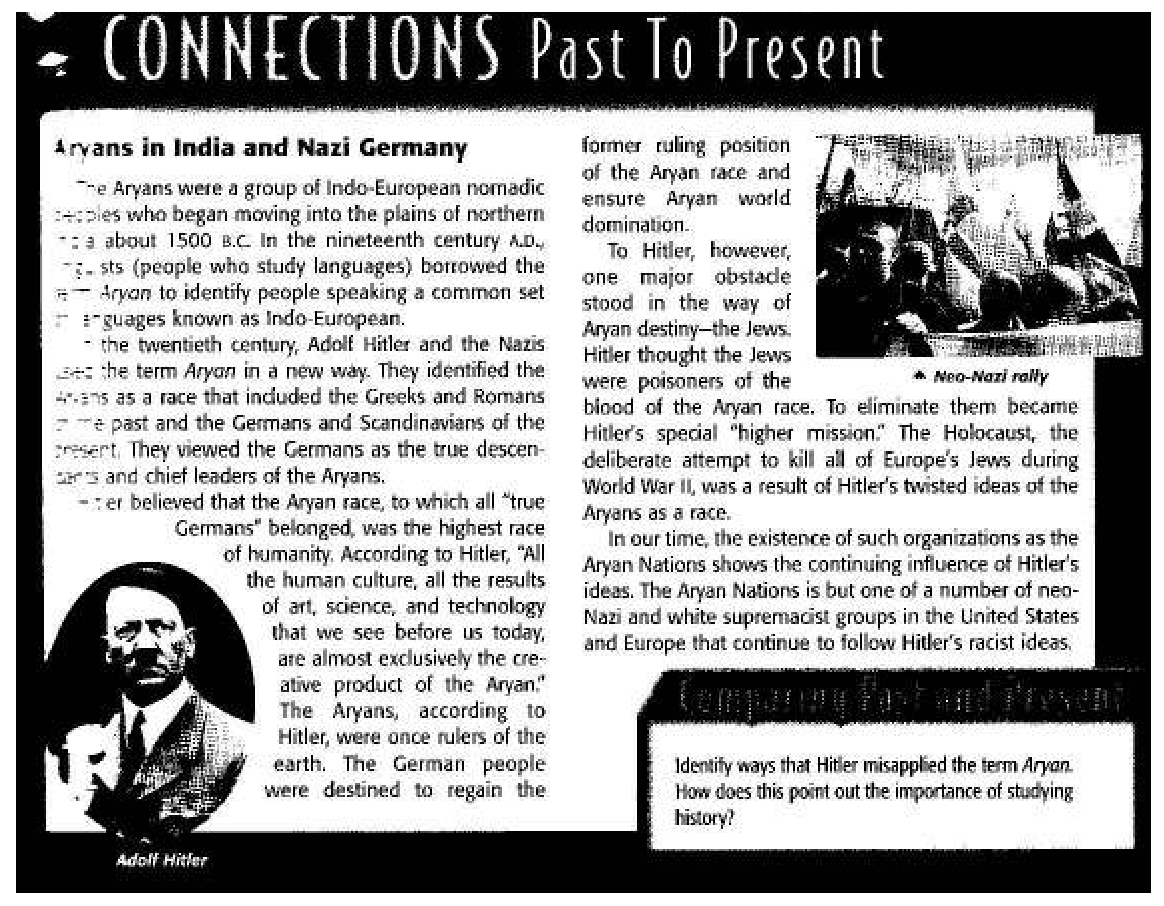
\includegraphics[scale=.21]{images/chap8-1.jpg}
\caption{A North Carolina school textbook (9th Grade) page from a chapter on Ancient India}\label{chap8-fig1}
\end{figure}


\section*{Bibliography}

\begin{thebibliography}{99}
\itemsep=0pt
\bibitem{chap8-key01} Adluri, Vishwa P. (2011). “Pride and Prejudice – Orientalism and German Indology.” \textit{International Journal of Hindu Studies.} Vol. 15, 3. pp 253--92.

 \bibitem{chap8-key02} Adluri, Vishwa and Joydeep Bagchee. (2015). “The Real Threat to Humanities Today” To be published in \textit{The International Journal of Hindu Studies}. (Draft version dt. October 10, 2015) available online at \url{https://www.academia.edu/18337993/The_Real_Threat_to_the_Humanities_Today_Andrew_Nicholson_The_Nay_Science_and_the_Future_of_Philology}. Accessed on 04 Jun 2016.

 \bibitem{chap8-key03} Agarwal, Vishal. (2004-5). “Misrepresentation and Stereotyping of Hindu Dharma in History Textbooks in India”. \textit{History Today} (New Delhi). Vol. 5. pp 60--76.

 \bibitem{chap8-key04} Asgharzadeh, Alireza. (2007). \textit{Iran and the Challenge of Diversity. }New York: Palgrave.

 \bibitem{chap8-key05} Bergman, Jerry. (2012). \textit{Hitler and the Nazi Darwinian Worldview.} Kitchener (Ontario): Joshua Press.

 \bibitem{chap8-key06} Breckenridge, Carol A. and van der Veer, Peter. (Eds.)(1993). \textit{Orientalism and the Postcolonial Predicament: Perspectives on South Asia}. South Asia Seminar Series. Philadelphia: University of Pennsylvania Press.

 \bibitem{chap8-key07} Burleigh, Michael and Wolfgang Wippermann. (1997). “Hitler’s Racism”. In Mitchell (1997). pp 83--87.

 \bibitem{chap8-key08} Chakrabarti, Dilip K. (1999). \textit{India- An Archaeological History, Paleolithic Beginnings to Early Historic Foundations}. New Delhi: Oxford University Press.

 \bibitem{chap8-key09} Chaubey, B. B. (1993). “Does the Word Arya in the Rgveda Connote a Race?”. \textit{Annals of the Bhandarkar Oriental Research Institute}, Vol. 42-43. pp 181--193.

 \bibitem{chap8-key10} Chitalwala. Y. M. (1984). “The Problem of Class Structure in the Indus Civilization”. In Lal and Gupta (1984). pp. 211--215.

 \bibitem{chap8-key11} Cornwell, John. (2000). \textit{Hitler’s Pope. }New York: Penguin Books.

 \bibitem{chap8-key12} —. (2003). \textit{Hitler’s Scientists.} New York: Viking.

 \bibitem{chap8-key13} Day, John. (2001). \textit{Indo-European Origins: The Anthropological Evidence.} Washington DC: The Institute for the Study of Man.

 \bibitem{chap8-key14} Deshpande, Madhav. (2006). “Aryan Origins, Brief History of Linguistic Arguments.” In Thapar \textit{et al.} (2006). pp 98--156.

 \bibitem{chap8-key15} Diaz-Andreu, Margarita. (1996). “Constructing Identities Through Culture”. In Graves-Brown \textit{et al.} pp 48--61.

 \bibitem{chap8-key16} Graves-Brown, Paul., Jones, Sian., and Gamble, Clive. (Ed.s). \textit{Cultural Identity and Archaeology – The Construction of European Communities}. London/New York: Routledge.

 \bibitem{chap8-key17} Elst, Koenraad. (1999). \textit{Update on the Aryan Invasion Debate. }Delhi: Aditya Prakashan.

 \bibitem{chap8-key18} —. (2001). \textit{Saffron Swastika. }Delhi: Voice of India.

 \bibitem{chap8-key19} Erdosy, George. (1989). “Ethnicity in the Rigveda and its Bearing on the Question of Indo-European Origins”. \textit{South Asian Studies}, Vol. 5. pp 35--47.

 \bibitem{chap8-key20} —. (Ed.) (1995). \textit{Indian Philology and South Asian Studies Vol. 1}. \textit{The Indo-Aryans of Ancient South Asia} - \textit{Language, Material Culture and Ethnicity. } Berlin/New York: de Gruyter.

 \bibitem{chap8-key21} Fitzgerald, Michael. (2013). \textit{The Nazi Occult War. }New York: Metro Books.

 \bibitem{chap8-key22} Halbfass, Wilhem. (1988). \textit{India and Europe, An Essay in Understanding}. Albany (New York): State University of New York Press.

 \bibitem{chap8-key23} Hamburger, F. (1952). “National-Socialism and Medicine”. In \textit{Readings on Fascism and National Socialism}; pp 108--110. Athens (Ohio, USA): Swallow Press.

 \bibitem{chap8-key24} Kater, Michael. (1989). \textit{Doctors under Hitler.} Chapel Hill: The University of North Carolina Press.

 \bibitem{chap8-key25} Kennedy, Kenneth A. R. (2000). \textit{God-Apes and Fossil Men, Paleoanthropology of South Asia}. Ann Arbor: The University of Michigan Press.

 \bibitem{chap8-key26} Kenoyer, Jonathan. (1998). \textit{Ancient Cities of the Indus Civilizatio}n. Karachi: Oxford University Press.

 \bibitem{chap8-key27} Lal, B. B., Gupta, S. P., and Asthana, S. (Ed.s) (1984).\textit{ Frontiers of the Indus Civilization}. New Delhi: Books \& Books on behalf of Indian Archaeological Society jointly with Indian History \& Culture Society.

 \bibitem{chap8-key28} Levitt, Stephen H. (1989). “What does ‘Noseless’ mean in the Rgveda”. \textit{The Annals Bhandarkar Oriental Research Institute.} Vol. 70, pp. 47--63.

 \bibitem{chap8-key29} Mair, Victor. (1998). “Priorities”. In Mair (1998a). pp 4--41.

 \bibitem{chap8-key30} —. (Ed.) (1998a). \textit{The Bronze Age and Early Iron Age Peoples of Eastern Central Asia}, Vol. I. (Journal of the Indo-European Studies Monograph No. 26). Washington D.C.: The Institute for the Study of Man (in collaboration with the University of Pennsylvania Museum Publications, Philadelphia).

\newpage

 \bibitem{chap8-key31} Malhotra, Rajiv. (2016). \textit{The Battle for Sanskrit}. Noida: Harper Collins.

 \bibitem{chap8-key32} McGetchin, Douglas T., Park, Peter K. J., and Sardesai, D. R. (Eds.) (2004). \textit{Sanskrit and ‘Orientalism’, Indology and Comparative Linguistics in German, 1750-1958}. New Delhi: Manohar Books.

 \bibitem{chap8-key33} Mīmāṁsaka, Yudhiṣṭhira. (1987-1993). \textit{Ācārya Śabarasvāmi-viracitam Jaiminīya Mīmāṁsā Bhāṣyam} (Vol. I-VII). Ramlal Kapoor Trust: Sonepat

 \bibitem{chap8-key34} Minkowski, Christopher. (1989). “The Rathakara’s Eligibility to Sacrifice”. \textit{Indo-Iranian Journal}. Vol. 32:3. pp 177--194.

 \bibitem{chap8-key35} Mitchell, Allan (Ed.) (1997). \textit{The Nazi Revolution}. Boston: Houghton Mifflin Company.

 \bibitem{chap8-key36} Murphy, Raymond E., Stevens, Francis., Trivers, Howard., and Roland, Joseph. (1952). “National Socialism”. In \textit{Readings on Fascism and National Socialism}. pp 62--107. Athens (Ohio, USA): Swallow Press.

 \bibitem{chap8-key37} Nath, Jyotish. (1996). \textit{The Dasas, Dasyus and Raksases in the Ṛgvedic Literature.} Calcutta: Sanskrit Pustak Bhandar.

 \bibitem{chap8-key38} Neubert, Frank. (2004). “Innovation Amid Controversy: Indology at Leipzig, 1841-1958”. In McGetchin \textit{et al.} (2004). pp 173--196.

 \bibitem{chap8-key39} Poewe, Karla., and Hexham, Irving. (2015). “Surprising Aryan Mediations between German Indology and Nazism”. \textit{International Journal of Hindu Studies}, Vol. 19:3. pp 263--300.

 \bibitem{chap8-key40} Poliakov, Leon. (1974). \textit{The Aryan Myth.} London: Sussex University Press.

 \bibitem{chap8-key41} Pollock, Sheldon. (1993). “Deep Orientalism?: Notes on Sanskrit and Power Beyond the Raj”. In Breckenridge and van der Veer (1993)\textit{. }pp 77--133.

\bibitem{chap8-key41a} \textbf{\textit{Śābara-bhāṣya.}} See Mīmāṁsaka (1987).

 \bibitem{chap8-key42} Schetelich, Maria. (1990). “The Problem of the ‘Dark Skin’ (Kṛṣṇa Tvac) in the Ṛgveda”. \textit{Visva Bharati Annals}. Vol. 3. pp. 244--249.
 
 \bibitem{chap8-key43} Sharma, Arvind. (2000). “Of Śūdras, Sūtas, and Ślokas: Why is the Mahābhārata Preeminently in the Anustubh Metre?”. \textit{The Indo-Iranian Journal}, Vol. 43. pp 225--278.

 \bibitem{chap8-key44} —. (Ed.) (2001). \textit{Hinduism and Secularism after Ayodhya}. New York: Palgrave.

 \bibitem{chap8-key45} Sharma, Ram Sharan. (2002). \textit{Śūdra-s in Ancient India.} New Delhi: Motilal Banarsidass.

 \bibitem{chap8-key46} Shastri, Ramgopalji. (1985). \textit{Kyā Veda Mein Āryon Aur Ādivāsiyon ke Yuddhon ka Varṇan Hai?} Sonepat: Ramlal Kapoor Trust.

 \bibitem{chap8-key47} Spielvogel, Jackson J. (1996). \textit{Hitler and Nazi Germany.} New Jersey: Prentice Hall.

 \bibitem{chap8-key48} Talageri, Shrikant G. (2000). \textit{The Rigveda – A Historical Analysis.} Delhi: Aditya Prakashan.

 \bibitem{chap8-key49} Thapar, Romila., Kenoyer, J. M., Deshpande, M. M., and Ratnagar, S. (2006). \textit{India: Historical Beginnings and the Concept of the Aryan. }New Delhi: National Book Trust.

 \bibitem{chap8-key50} Tilak, Shrinivas. (2001). “Hindutva – the Indian Secularists’ Metaphor for illness and Perversion”. In Sharma (2001)\textit{.} pp 123--134.

 \bibitem{chap8-key51} Venkat, Kalavai. (2007). “From the Holy Cross to the Holocaust”. In \textit{Expressions of Christianity}. pp 153--204. Chennai: Vivekananda Kendra Prakashan Trust.

 \bibitem{chap8-key52} Wakankar, Vishnu Shridhar. (1988). \textit{Vaidik Arya Samasya}. Noida: Jagriti Prakashan.

 \bibitem{chap8-key53} Witzel, Michael. (1995). “Ṛgvedic History: Poets, Chieftains and Politics”. In Erdosy (1995). pp 307--352.

 \bibitem{chap8-key54} —., Lubotsky, A., Oort, M. S. (Ed.s) (1997). \textit{F. B. J. Kuiper- Selected Writings on Indian Linguistics and Philology}. Amsterdam/Atlanta: Rodopi.

 \end{thebibliography}

\theendnotes

\label{chapter8-end}
